\documentclass[border=4pt]{standalone}
\usepackage{tikz,amsmath}
\usetikzlibrary{arrows.meta}
\definecolor{nuit}{HTML}{190F3C}\definecolor{bleu}{HTML}{3746FF}
\definecolor{corail}{HTML}{FF808B}\definecolor{corailf}{HTML}{D6455A}
\definecolor{bleuclair}{HTML}{9BA3FF}
\newcommand{\vv}[1]{\underline{#1}}
\begin{document}
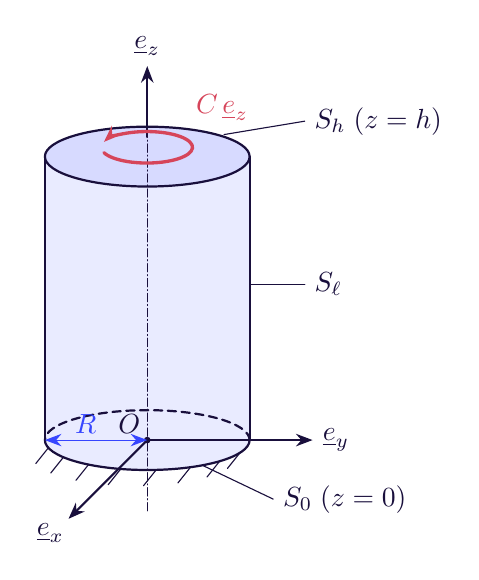
\begin{tikzpicture}[line cap=round,line join=round,>={Stealth[length=6pt]},
  every node/.style={text=nuit}]
  \def\R{1.3}\def\r{0.38}\def\H{3.6}
  % Remplissage du barreau
  \fill[bleuclair!22] (-\R,0) -- (-\R,\H) arc[start angle=180,end angle=360,x radius=\R,y radius=\r]
        -- (\R,0) arc[start angle=0,end angle=-180,x radius=\R,y radius=\r] -- cycle;
  \fill[bleuclair!40] (0,\H) ellipse[x radius=\R,y radius=\r];
  % Contour
  \draw[nuit,thick] (-\R,0) -- (-\R,\H) (\R,0) -- (\R,\H);
  \draw[nuit,thick] (0,\H) ellipse[x radius=\R,y radius=\r];
  \draw[nuit,thick] (\R,0) arc[start angle=0,end angle=-180,x radius=\R,y radius=\r];
  \draw[nuit,thick,densely dashed] (\R,0) arc[start angle=0,end angle=180,x radius=\R,y radius=\r];
  % Encastrement sur S_0
  \foreach \t in {195,215,...,345}{
    \draw[nuit] ({\R*cos(\t)},{\r*sin(\t)}) -- ++(-0.16,-0.2);}
  % Axes
  \draw[nuit,densely dash dot] (0,-0.9) -- (0,\H+0.25);
  \draw[->,nuit,thick] (0,\H+0.25) -- (0,\H+1.15) node[above] {$\vv{e}_z$};
  \draw[->,nuit,thick] (0,0) -- (2.1,0) node[right] {$\vv{e}_y$};
  \draw[->,nuit,thick] (0,0) -- (-1.0,-1.0) node[below left=-2pt] {$\vv{e}_x$};
  \fill[nuit] (0,0) circle (1.2pt) node[above left=-1pt] {$O$};
  % Couple sur S_h
  \draw[->,corailf,very thick] (-0.55,\H+0.05) arc[start angle=200,end angle=520,x radius=0.58,y radius=0.2];
  \node[text=corailf] at (0.95,\H+0.62) {$C\,\vv{e}_z$};
  % Noms des surfaces
  \draw[nuit] (\R*0.75,\H+0.28) -- (2.0,\H+0.45) node[right] {$S_h \;(z=h)$};
  \draw[nuit] (\R,0.55*\H) -- (2.0,0.55*\H) node[right] {$S_\ell$};
  \draw[nuit] (0.7,-0.32) -- (1.6,-0.75) node[right] {$S_0 \;(z=0)$};
  % Rayon
  \draw[<->,bleu] (0,0) -- (-\R,0) node[pos=0.6,above=-1pt,text=bleu] {$R$};
\end{tikzpicture}
\end{document}
